%!TEX root = ../../../super_main.tex

\section{Reengineering the Application Grid}
\label{sec:reengineering_of_application_grid}

When the \launcher of the \giraf system is being used, and the user presses the drawer on the left-hand side (see \figrefpage{fig:initial_launcher}), the application container becomes smaller as a result of the drawer moving on the screen. The resulting smaller area has to be repopulated with icons, since the icons are no longer within the boundaries of the screen. Furthermore, the application window currently has a fixed size, while the user is able to select as many applications as he/she wants. This means that if too many applications are chosen, they will surpass the size of the window, and therefore be pushed out of the window as seen in \figref{fig:overflow_problem}. The applications are currently being placed in the \launcher by using \androidinline{LinearLayout}s placed in rows, which then individually contain an amount of icons respective to the icon size. This has a serious effect on performance and smoothness of the \launcher. 

\begin{figure}[!htbp]
    \centering
    \begin{subfigure}[t]{0.3\textwidth}
        \centering
        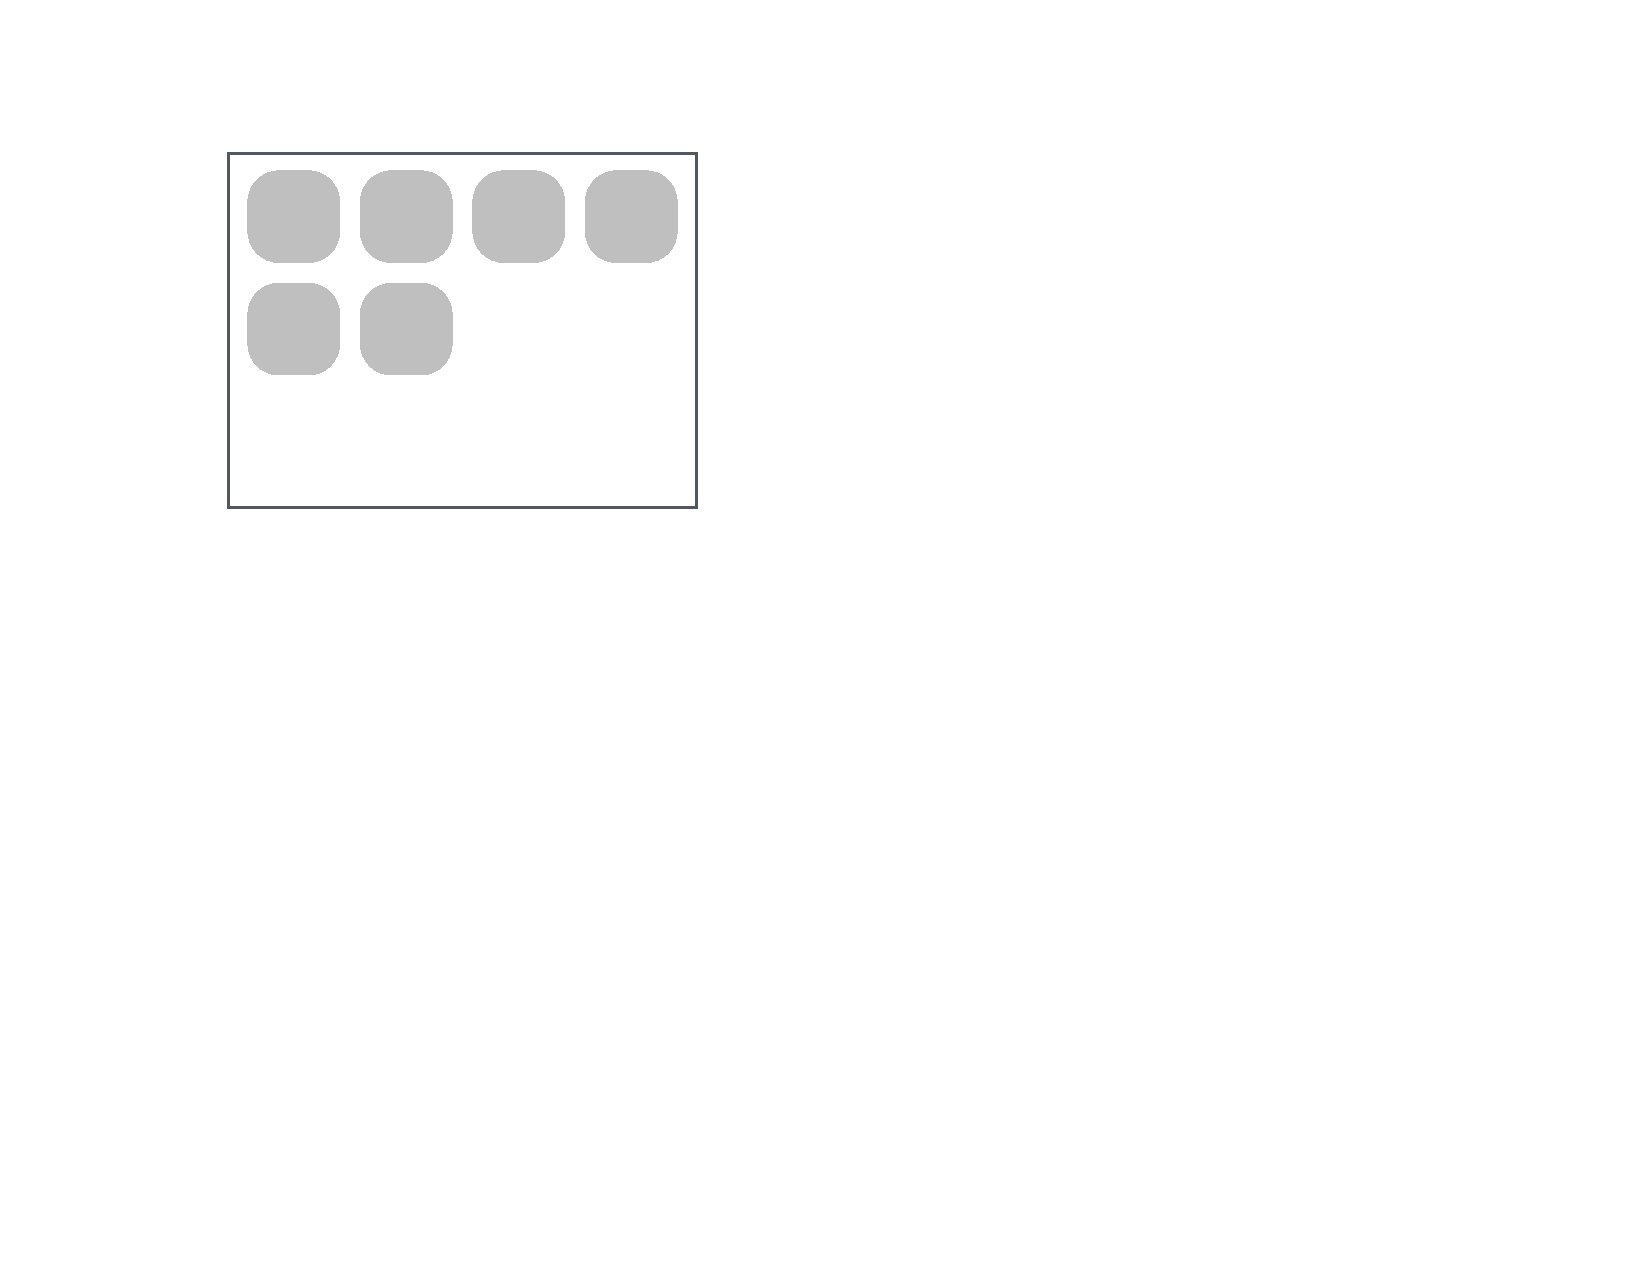
\includegraphics[width=0.7\textwidth]{sprint_one/reengineering_of_application_grid/overflow_problem_small}
        \caption{Small sized application icons}
        \label{fig:overflow_problem_small}
    \end{subfigure}
    \hspace{5em} 
    \begin{subfigure}[t]{0.3\textwidth}
        \centering
        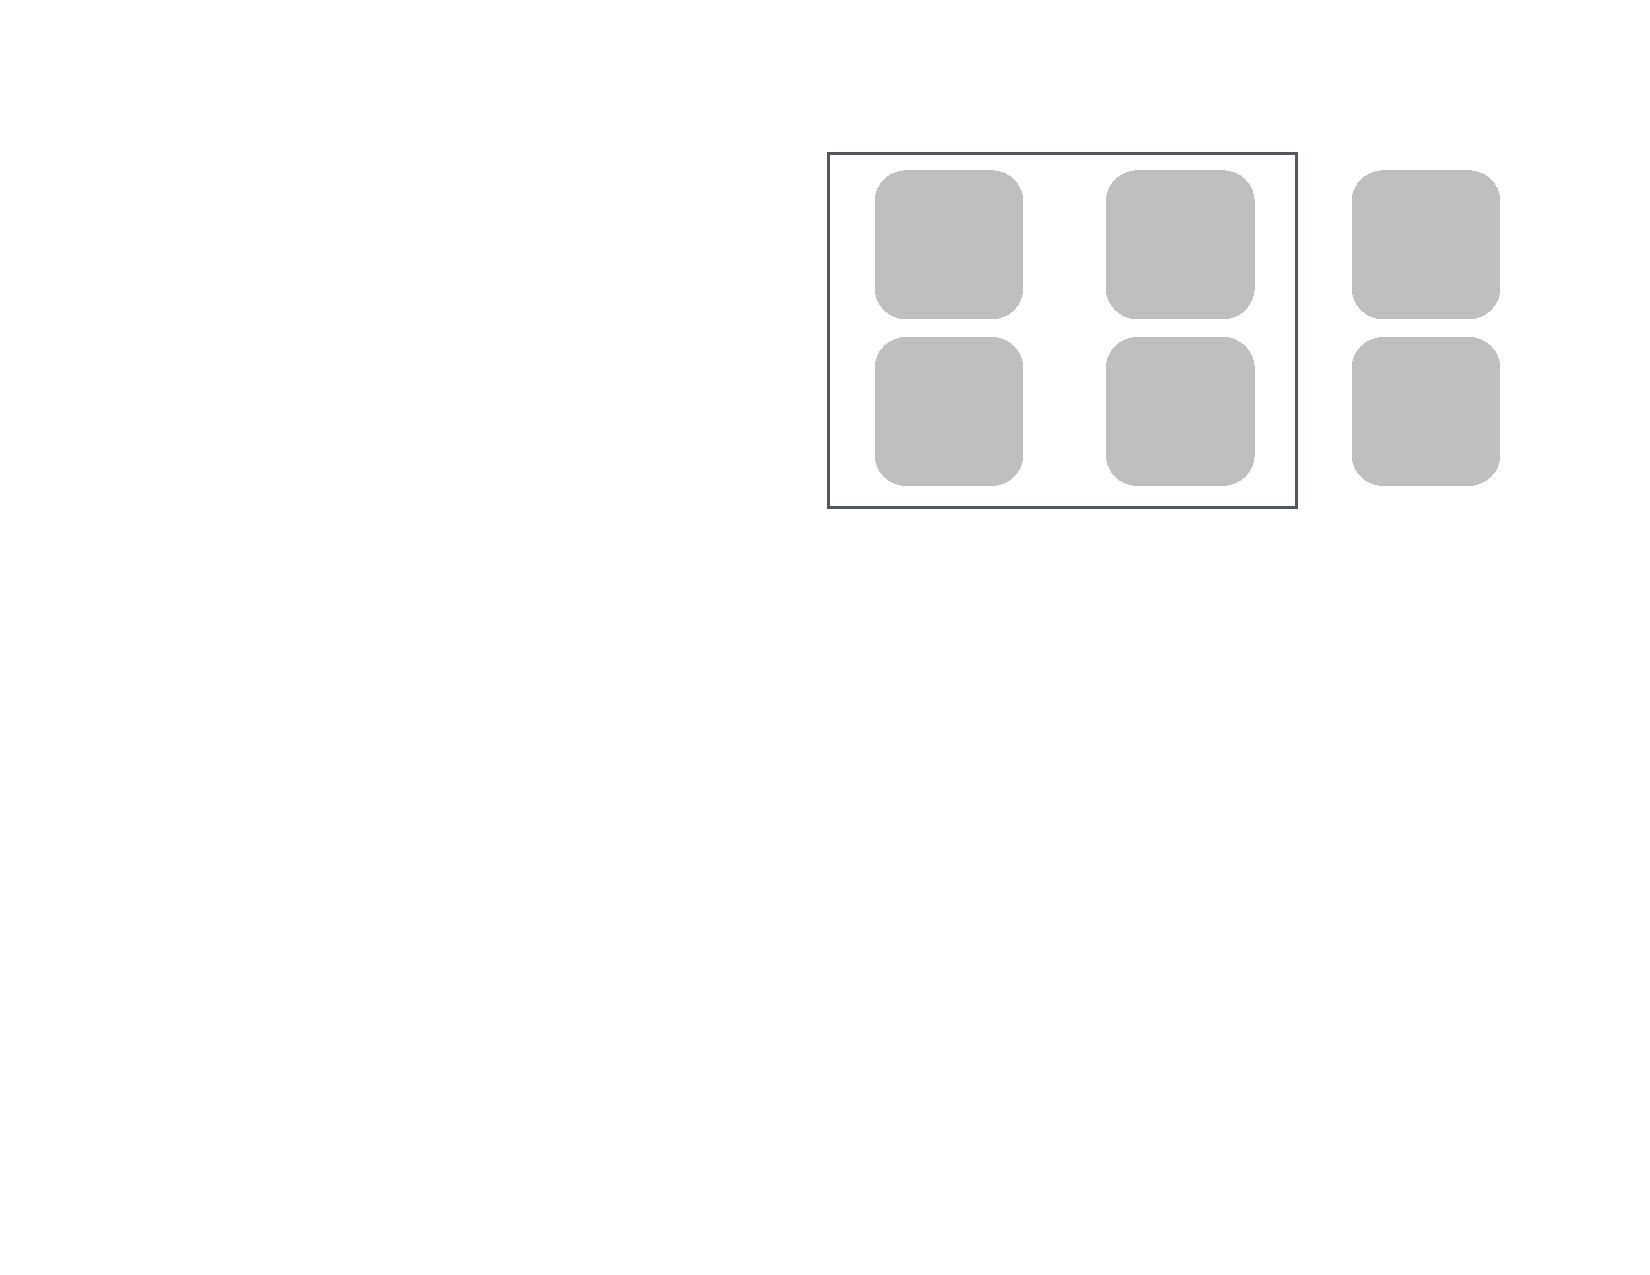
\includegraphics[width=\textwidth]{sprint_one/reengineering_of_application_grid/overflow_problem_large}
        \caption{Large sized application icons}
        \label{fig:overflow_problem_large}
    \end{subfigure}
    
    \caption{Overflow of application icons}
    \label{fig:overflow_problem}
\end{figure}

\FloatBarrier

The application grid has a setting in the settings menu which allows the user to configure the icon size of the applications shown in the \launcher. The icon size is adjusted by pulling the \androidinline{SeekBar} (slider). This settings menu can be seen in \figref{fig:preference_screen_old}.

\begin{figure}[!htbp]
    \centering
    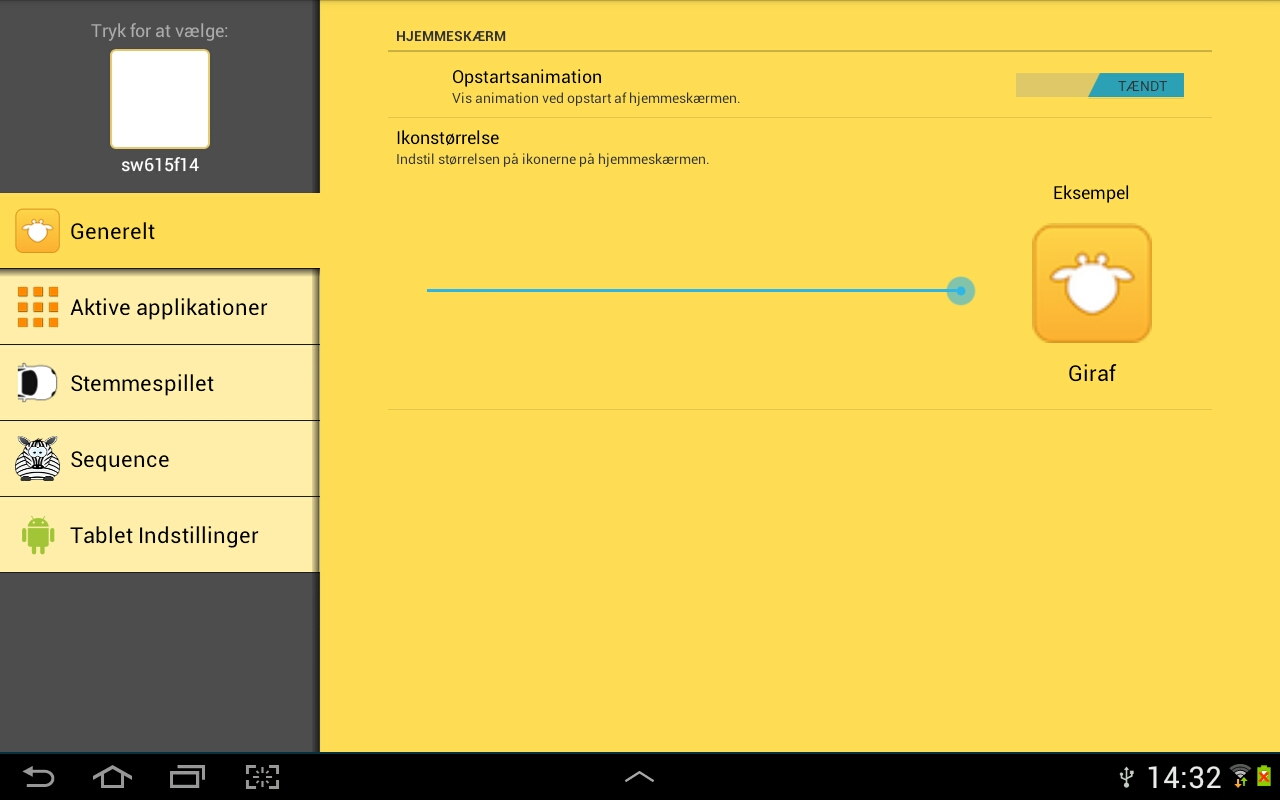
\includegraphics[width=\textwidth]{sprint_one/reengineering_of_application_grid/preference_screen_old}
    \caption{Old preference screen}
    \label{fig:preference_screen_old}
\end{figure}

The \androidinline{LinearLayout} views that are created fit as many icons of the given size inside as possible, while staying within the width of the screen. This is some ``hack'' method that has been implemented in order to allow users to manually change how many icons they want to see in the \launcher. This solution is bad, because instead of changing the actual amount of icons on the screen, the items are just scaled down so more of them can fit on the screen with no indication of how many icons you will now see. Note that this feature was implemented per request of the users, which means that the scaling cannot simply be removed. Instead it motivated us to create a better solution.
\\\\
The creation of \androidinline{LinearLayout} views gave the user a poor experience when interacting with the application, and we have therefore improved the \launcher application such that it uses a \androidinline{ViewPager} which contains a grid structure instead. An implementation using \androidinline{GridLayout} is preferable compared to rows of \androidinline{LinearLayout} views, since it is easier to build and populate with icons, which should result in increased performance. A \androidinline{ViewPager} is the standard way of allowing the user to page between screens of applications in other \launcher activities, which is desirable since it gives the user a consistent experience with comparable devices they use. Furthermore, a \androidinline{ViewPagerIndicator} is added to the bottom of the screen, so users have a clear overview of how many pages of applications there are, and how far they have progressed in the paging. The implemented \androidinline{ViewPagerIndicator} comes from an external library \parencite{view_pager_indicator_avianey}, since there is no standard implementation of such a widget in Android.
\\\\
The functionality in the settings menu that allowed users to change the size of icons has been replaced with the possibility of changing the \launcher grid size. The icon preview in the settings menu now shows an example grid instead. The new setting allows the user to change the size of the grid directly, instead of using the aforementioned indirect icon-resize method. The new settings menu can be seen in \figref{fig:preference_screen_new}.

\todo{Write about the limitation of this settings, we have preset amount of settings. Also mention that we considered two sliders.}

\begin{figure}[!htbp]
    \centering
    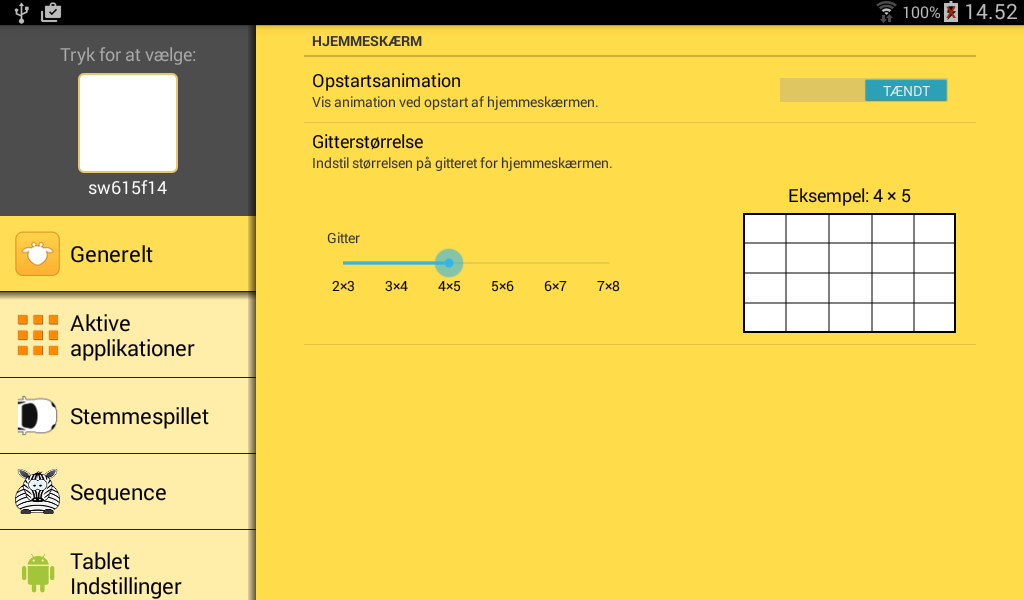
\includegraphics[width=\textwidth]{sprint_one/reengineering_of_application_grid/preference_screen_new}
    \caption{New preference screen}
    \label{fig:preference_screen_new}
\end{figure}